\newcommand*{\ptsans}{\fontfamily{PTSans-TLF}\selectfont}    % toggle to change to the standard font of the University of Kaiserslautern: PT Sans
\DeclareTextFontCommand{\textptsans}{\ptsans}                % environment to change to the standard font of the University of Kaiserslautern: PT Sans

\definecolor{TUblue}{RGB}{0,96,142}     % The blue color used in the logo of the University of Kaiserslautern
\definecolor{TUred}{RGB}{188,38,26}     % The red color used in the logo of the University of Kaiserslautern

% The following new commands are tikzpicture-environments containing different logos of the University of Kaiserslautern. They are taken from logos published on their website.
% It defines the following commands: \TULogo, \TULogoWithText, \CSLogo

% The logo of the University of Kaiserslautern ():
% Taken from: http://www.uni-kl.de/fileadmin/prum/tupublic/TU_Logo_ohne_Feld/TUKL_LOGO_4C.svg on the 2016-12-14
% Manipulated using: Inkscape (https://inkscape.org/)
% Converted to TikZ using: svg2tikz (https://github.com/kjellmf/svg2tikz) as an Inkscape extension
\newcommand{\TULogo}[1][1]{
    \begin{tikzpicture}[
        y = 5pt,
        x = 5pt,
        opacity = #1
    ]
        % Top part:
        \path[fill = TUblue] (2.898, 23.855) -- (2.898, 20.561) -- (24.299, 20.561)  -- (24.299, 24.034) -- (13.541, 27.197) -- cycle;
        % Left part:
        \path[fill = TUblue] (5.679, 19.307) -- (9.993, 19.307) -- (4.3, 0)  -- (0, 0) -- cycle;
        % Top rectangle:
        \path[fill = TUblue] (17.481, 19.316) rectangle (22.247, 14.727);
        % Middle rectangle:
        \path[fill = TUred] (17.481, 11.953) rectangle (22.247, 7.363);
        % Bottom rectangle:
        \path[fill = TUblue] (17.481, 4.59) rectangle (22.247, 0);
    \end{tikzpicture}
}

% The logo with text of the University of Kaiserslautern:
% Taken from: http://www.uni-kl.de/fileadmin/prum/tupublic/TU_Logo_ohne_Feld/TUKL_LOGO_4C.svg on the 2016-12-14
% Converted to TikZ using: svg2tikz (https://github.com/kjellmf/svg2tikz) as an Inkscape (https://inkscape.org/) extension
\newcommand{\TULogoWithText}{
    
\begin{tikzpicture}[
        y = 0.8pt,
        x = 0.8pt,
        yscale = -1,
        xscale = 1
    ]
        % KAISERSLAUTERN:
        \path[fill = TUblue] (164.0310,41.3410) -- (164.0310,36.5480) -- (163.8200,35.1050) -- (163.8890,35.1050) -- (164.6070,36.5480) -- (168.0610,41.4050) -- (169.3700,41.4050) -- (169.3700,32.1510) -- (167.6650,32.1510) -- (167.6650,36.9830) -- (167.8760,38.3870) -- (167.8120,38.3870) -- (167.1170,36.9810) -- (163.6440,32.0860) -- (162.3270,32.0860) -- (162.3270,41.3400) -- (164.0310,41.3400) -- cycle(155.4790,33.6880) .. controls (155.5790,33.6630) and (155.7170,33.6450) .. (155.8970,33.6370) .. controls (156.0780,33.6290) and (156.2590,33.6250) .. (156.4440,33.6250) .. controls (156.9200,33.6250) and (157.2800,33.7360) .. (157.5230,33.9570) .. controls (157.7670,34.1800) and (157.8890,34.4880) .. (157.8890,34.8810) .. controls (157.8890,35.4060) and (157.7410,35.7830) .. (157.4420,36.0120) .. controls (157.1450,36.2410) and (156.7460,36.3540) .. (156.2450,36.3540) -- (155.4790,36.3540) -- (155.4790,33.6880) -- cycle(155.4790,41.3410) -- (155.4790,37.5730) -- (156.4560,37.7820) -- (158.5240,41.3410) -- (160.5940,41.3410) -- (158.5110,37.8720) -- (157.8510,37.4330) .. controls (158.3790,37.2490) and (158.8020,36.9190) .. (159.1200,36.4470) .. controls (159.4350,35.9720) and (159.5950,35.3570) .. (159.5950,34.6050) .. controls (159.5950,34.1010) and (159.5020,33.6810) .. (159.3150,33.3430) .. controls (159.1290,33.0070) and (158.8800,32.7410) .. (158.5680,32.5480) .. controls (158.2570,32.3570) and (157.9040,32.2200) .. (157.5090,32.1420) .. controls (157.1140,32.0620) and (156.7140,32.0230) .. (156.3090,32.0230) .. controls (156.1320,32.0230) and (155.9380,32.0290) .. (155.7270,32.0370) .. controls (155.5160,32.0450) and (155.3000,32.0580) .. (155.0780,32.0760) .. controls (154.8540,32.0920) and (154.6310,32.1170) .. (154.4050,32.1480) .. controls (154.1790,32.1810) and (153.9700,32.2140) .. (153.7770,32.2480) -- (153.7770,41.3420) -- (155.4790,41.3420) -- cycle(151.9100,41.3410) -- (151.9100,39.7390) -- (148.1030,39.7390) -- (148.1030,37.4970) -- (151.5180,37.4970) -- (151.5180,35.8930) -- (148.1030,35.8930) -- (148.1030,33.7520) -- (151.8450,33.7520) -- (151.8450,32.1500) -- (146.3980,32.1500) -- (146.3980,41.3390) -- (151.9100,41.3390) -- cycle(140.2020,33.7530) -- (140.2020,41.3410) -- (141.9070,41.3410) -- (141.9070,33.7530) -- (144.6810,33.7530) -- (144.6810,32.1510) -- (137.4200,32.1510) -- (137.4200,33.7530) -- (140.2020,33.7530) -- cycle(132.7710,41.5010) .. controls (133.2500,41.5010) and (133.6930,41.4350) .. (134.0960,41.3040) .. controls (134.5000,41.1710) and (134.8420,40.9640) .. (135.1220,40.6850) .. controls (135.4020,40.4060) and (135.6200,40.0500) .. (135.7770,39.6210) .. controls (135.9320,39.1910) and (136.0100,38.6800) .. (136.0100,38.0860) -- (136.0100,32.1520) -- (134.3050,32.1520) -- (134.3050,37.9590) .. controls (134.3050,38.6390) and (134.1820,39.1310) .. (133.9360,39.4390) .. controls (133.6890,39.7460) and (133.2900,39.9000) .. (132.7390,39.9000) .. controls (132.4610,39.9000) and (132.2170,39.8670) .. (132.0070,39.8000) .. controls (131.7970,39.7330) and (131.6220,39.6240) .. (131.4800,39.4700) .. controls (131.3390,39.3160) and (131.2360,39.1160) .. (131.1690,38.8680) .. controls (131.1020,38.6200) and (131.0700,38.3150) .. (131.0700,37.9580) -- (131.0700,32.1510) -- (129.3650,32.1510) -- (129.3650,38.3090) .. controls (129.3660,40.4370) and (130.5010,41.5010) .. (132.7710,41.5010)(123.9030,35.8310) -- (124.1770,34.3760) -- (124.2410,34.3760) -- (124.5220,35.8170) -- (125.2030,37.8620) -- (123.2280,37.8620) -- (123.9030,35.8310) -- cycle(122.0790,41.3410) -- (122.7000,39.4640) -- (125.7220,39.4640) -- (126.3310,41.3410) -- (128.0350,41.3410) -- (124.7280,32.0870) -- (123.4420,32.0870) -- (120.2810,41.3410) -- (122.0790,41.3410) -- cycle(119.2220,41.3410) -- (119.2220,39.7390) -- (115.1150,39.7390) -- (115.1150,32.1510) -- (113.4100,32.1510) -- (113.4100,41.3400) -- (119.2220,41.3400) -- cycle(106.5570,41.3410) .. controls (107.0430,41.4640) and (107.6040,41.5290) .. (108.2410,41.5290) .. controls (108.7220,41.5290) and (109.1670,41.4700) .. (109.5720,41.3530) .. controls (109.9760,41.2380) and (110.3220,41.0600) .. (110.6060,40.8240) .. controls (110.8910,40.5880) and (111.1130,40.2910) .. (111.2700,39.9330) .. controls (111.4280,39.5760) and (111.5070,39.1480) .. (111.5070,38.6540) .. controls (111.5070,38.1770) and (111.4160,37.7790) .. (111.2330,37.4570) .. controls (111.0510,37.1350) and (110.8230,36.8650) .. (110.5450,36.6460) .. controls (110.2680,36.4290) and (109.9500,36.2380) .. (109.5900,36.0740) .. controls (109.2310,35.9080) and (108.8940,35.7540) .. (108.5810,35.6110) .. controls (108.2680,35.4680) and (107.9950,35.3080) .. (107.7620,35.1360) .. controls (107.5300,34.9620) and (107.4120,34.7470) .. (107.4120,34.4880) .. controls (107.4120,34.2090) and (107.5230,33.9880) .. (107.7470,33.8220) .. controls (107.9690,33.6580) and (108.2910,33.5760) .. (108.7110,33.5760) .. controls (109.1480,33.5760) and (109.5540,33.6250) .. (109.9300,33.7220) .. controls (110.3050,33.8240) and (110.5860,33.9330) .. (110.7740,34.0540) -- (111.3070,32.5250) .. controls (111.0130,32.3450) and (110.6360,32.2090) .. (110.1770,32.1150) .. controls (109.7170,32.0190) and (109.2280,31.9720) .. (108.7110,31.9720) .. controls (108.2630,31.9720) and (107.8570,32.0250) .. (107.4920,32.1300) .. controls (107.1270,32.2370) and (106.8100,32.4000) .. (106.5440,32.6200) .. controls (106.2780,32.8400) and (106.0700,33.1180) .. (105.9250,33.4500) .. controls (105.7800,33.7840) and (105.7080,34.1750) .. (105.7080,34.6240) .. controls (105.7080,35.1340) and (105.8100,35.5540) .. (106.0150,35.8840) .. controls (106.2200,36.2120) and (106.4790,36.4880) .. (106.7910,36.7060) .. controls (107.1030,36.9250) and (107.4380,37.1140) .. (107.7990,37.2740) .. controls (108.1600,37.4340) and (108.4950,37.5830) .. (108.8080,37.7210) .. controls (109.1210,37.8620) and (109.3660,38.0140) .. (109.5400,38.1840) .. controls (109.7140,38.3540) and (109.8030,38.5790) .. (109.8030,38.8540) .. controls (109.8030,39.2150) and (109.6600,39.4830) .. (109.3760,39.6610) .. controls (109.0910,39.8370) and (108.6810,39.9250) .. (108.1450,39.9250) .. controls (107.9260,39.9250) and (107.7140,39.9090) .. (107.5080,39.8740) .. controls (107.3010,39.8410) and (107.1050,39.7980) .. (106.9200,39.7450) .. controls (106.7330,39.6920) and (106.5660,39.6360) .. (106.4190,39.5750) .. controls (106.2700,39.5130) and (106.1480,39.4580) .. (106.0540,39.4070) -- (105.4770,40.9620) .. controls (105.7110,41.0890) and (106.0710,41.2160) .. (106.5570,41.3410)(99.0840,33.6880) .. controls (99.1830,33.6630) and (99.3220,33.6450) .. (99.5020,33.6370) .. controls (99.6820,33.6290) and (99.8640,33.6250) .. (100.0480,33.6250) .. controls (100.5230,33.6250) and (100.8830,33.7360) .. (101.1270,33.9570) .. controls (101.3720,34.1800) and (101.4940,34.4880) .. (101.4940,34.8810) .. controls (101.4940,35.4060) and (101.3450,35.7830) .. (101.0470,36.0120) .. controls (100.7490,36.2410) and (100.3500,36.3540) .. (99.8490,36.3540) -- (99.0840,36.3540) -- (99.0840,33.6880) -- cycle(99.0840,41.3410) -- (99.0840,37.5730) -- (100.0600,37.7820) -- (102.1280,41.3410) -- (104.1980,41.3410) -- (102.1160,37.8720) -- (101.4550,37.4330) .. controls (101.9840,37.2490) and (102.4070,36.9190) .. (102.7230,36.4470) .. controls (103.0400,35.9720) and (103.1990,35.3570) .. (103.1990,34.6050) .. controls (103.1990,34.1010) and (103.1050,33.6810) .. (102.9200,33.3430) .. controls (102.7330,33.0070) and (102.4850,32.7410) .. (102.1730,32.5480) .. controls (101.8610,32.3570) and (101.5080,32.2200) .. (101.1130,32.1420) .. controls (100.7180,32.0620) and (100.3190,32.0230) .. (99.9140,32.0230) .. controls (99.7360,32.0230) and (99.5420,32.0290) .. (99.3320,32.0370) .. controls (99.1210,32.0450) and (98.9040,32.0580) .. (98.6810,32.0760) .. controls (98.4580,32.0920) and (98.2340,32.1170) .. (98.0090,32.1480) .. controls (97.7840,32.1810) and (97.5740,32.2140) .. (97.3800,32.2480) -- (97.3800,41.3420) -- (99.0840,41.3420) -- cycle(95.2520,41.3410) -- (95.2520,39.7390) -- (91.4460,39.7390) -- (91.4460,37.4970) -- (94.8610,37.4970) -- (94.8610,35.8930) -- (91.4460,35.8930) -- (91.4460,33.7520) -- (95.1880,33.7520) -- (95.1880,32.1500) -- (89.7410,32.1500) -- (89.7410,41.3390) -- (95.2520,41.3390) -- cycle(82.6260,41.3410) .. controls (83.1120,41.4640) and (83.6730,41.5290) .. (84.3090,41.5290) .. controls (84.7910,41.5290) and (85.2350,41.4700) .. (85.6400,41.3530) .. controls (86.0450,41.2380) and (86.3900,41.0600) .. (86.6750,40.8240) .. controls (86.9590,40.5880) and (87.1810,40.2910) .. (87.3390,39.9330) .. controls (87.4970,39.5750) and (87.5760,39.1480) .. (87.5760,38.6540) .. controls (87.5760,38.1770) and (87.4840,37.7790) .. (87.3020,37.4570) .. controls (87.1200,37.1350) and (86.8900,36.8650) .. (86.6130,36.6460) .. controls (86.3360,36.4290) and (86.0180,36.2380) .. (85.6580,36.0740) .. controls (85.2990,35.9080) and (84.9620,35.7540) .. (84.6490,35.6110) .. controls (84.3360,35.4680) and (84.0630,35.3080) .. (83.8300,35.1360) .. controls (83.5970,34.9620) and (83.4800,34.7470) .. (83.4800,34.4880) .. controls (83.4800,34.2090) and (83.5920,33.9880) .. (83.8150,33.8220) .. controls (84.0370,33.6580) and (84.3590,33.5760) .. (84.7780,33.5760) .. controls (85.2160,33.5760) and (85.6220,33.6250) .. (85.9980,33.7220) .. controls (86.3730,33.8240) and (86.6540,33.9330) .. (86.8410,34.0540) -- (87.3750,32.5250) .. controls (87.0810,32.3450) and (86.7040,32.2090) .. (86.2450,32.1150) .. controls (85.7850,32.0190) and (85.2960,31.9720) .. (84.7780,31.9720) .. controls (84.3310,31.9720) and (83.9250,32.0250) .. (83.5600,32.1300) .. controls (83.1950,32.2370) and (82.8790,32.4000) .. (82.6120,32.6200) .. controls (82.3440,32.8410) and (82.1380,33.1180) .. (81.9930,33.4500) .. controls (81.8480,33.7840) and (81.7760,34.1750) .. (81.7760,34.6240) .. controls (81.7760,35.1340) and (81.8780,35.5540) .. (82.0830,35.8840) .. controls (82.2880,36.2120) and (82.5470,36.4880) .. (82.8590,36.7060) .. controls (83.1710,36.9240) and (83.5070,37.1140) .. (83.8670,37.2740) .. controls (84.2270,37.4340) and (84.5630,37.5830) .. (84.8760,37.7210) .. controls (85.1890,37.8620) and (85.4330,38.0140) .. (85.6080,38.1840) .. controls (85.7830,38.3540) and (85.8710,38.5790) .. (85.8710,38.8540) .. controls (85.8710,39.2150) and (85.7280,39.4830) .. (85.4430,39.6610) .. controls (85.1590,39.8370) and (84.7480,39.9250) .. (84.2130,39.9250) .. controls (83.9940,39.9250) and (83.7820,39.9090) .. (83.5760,39.8740) .. controls (83.3690,39.8410) and (83.1730,39.7980) .. (82.9880,39.7450) .. controls (82.8020,39.6920) and (82.6350,39.6360) .. (82.4870,39.5750) .. controls (82.3380,39.5130) and (82.2160,39.4580) .. (82.1210,39.4070) -- (81.5450,40.9620) .. controls (81.7800,41.0890) and (82.1400,41.2160) .. (82.6260,41.3410)(79.7610,32.1510) -- (78.0560,32.1510) -- (78.0560,41.3400) -- (79.7610,41.3400) -- (79.7610,32.1510) -- cycle(72.1060,35.8310) -- (72.3820,34.3760) -- (72.4460,34.3760) -- (72.7280,35.8170) -- (73.4070,37.8620) -- (71.4340,37.8620) -- (72.1060,35.8310) -- cycle(70.2820,41.3410) -- (70.9030,39.4640) -- (73.9260,39.4640) -- (74.5350,41.3410) -- (76.2400,41.3410) -- (72.9330,32.0870) -- (71.6470,32.0870) -- (68.4850,41.3410) -- (70.2820,41.3410) -- cycle(62.0580,41.3410) -- (62.0580,37.4560) -- (62.5690,37.4560) -- (65.2560,41.3410) -- (67.4730,41.3410) -- (64.4440,37.0620) -- (63.6760,36.5440) -- (64.3890,36.0480) -- (67.0700,32.1520) -- (65.0190,32.1520) -- (62.4820,36.0430) -- (62.0580,36.2210) -- (62.0580,32.1530) -- (60.3530,32.1530) -- (60.3530,41.3420) -- (62.0580,41.3420) -- cycle;
        % TECHNISCHE UNIVERSITÄT:
        \path[fill=TUred] (166.8350,23.1740) -- (166.8350,28.6690) -- (168.0690,28.6690) -- (168.0690,23.1740) -- (170.0790,23.1740) -- (170.0790,22.0140) -- (164.8210,22.0140) -- (164.8210,23.1740) -- (166.8350,23.1740) -- cycle(162.7020,21.4690) .. controls (162.8160,21.5720) and (162.9970,21.6240) .. (163.2450,21.6240) .. controls (163.4980,21.6240) and (163.6830,21.5720) .. (163.7950,21.4690) .. controls (163.9080,21.3650) and (163.9640,21.2260) .. (163.9640,21.0510) .. controls (163.9640,20.8740) and (163.9080,20.7310) .. (163.7950,20.6240) .. controls (163.6830,20.5170) and (163.4980,20.4640) .. (163.2450,20.4640) .. controls (162.9970,20.4640) and (162.8160,20.5180) .. (162.7020,20.6270) .. controls (162.5870,20.7350) and (162.5300,20.8770) .. (162.5300,21.0510) .. controls (162.5300,21.2260) and (162.5870,21.3650) .. (162.7020,21.4690)(160.6690,21.4690) .. controls (160.7840,21.5720) and (160.9680,21.6240) .. (161.2210,21.6240) .. controls (161.4660,21.6240) and (161.6460,21.5720) .. (161.7600,21.4690) .. controls (161.8740,21.3650) and (161.9320,21.2260) .. (161.9320,21.0510) .. controls (161.9320,20.8740) and (161.8750,20.7310) .. (161.7620,20.6240) .. controls (161.6500,20.5170) and (161.4690,20.4640) .. (161.2210,20.4640) .. controls (160.9680,20.4640) and (160.7840,20.5180) .. (160.6690,20.6270) .. controls (160.5560,20.7350) and (160.4970,20.8770) .. (160.4970,21.0510) .. controls (160.4970,21.2260) and (160.5560,21.3650) .. (160.6690,21.4690)(161.9410,24.6780) -- (162.1400,23.6240) -- (162.1870,23.6240) -- (162.3910,24.6680) -- (162.8820,26.1490) -- (161.4530,26.1490) -- (161.9410,24.6780) -- cycle(160.6200,28.6690) -- (161.0700,27.3090) -- (163.2580,27.3090) -- (163.6990,28.6690) -- (164.9330,28.6690) -- (162.5380,21.9670) -- (161.6060,21.9670) -- (159.3170,28.6690) -- (160.6200,28.6690) -- cycle(156.2580,23.1740) -- (156.2580,28.6690) -- (157.4920,28.6690) -- (157.4920,23.1740) -- (159.5020,23.1740) -- (159.5020,22.0140) -- (154.2440,22.0140) -- (154.2440,23.1740) -- (156.2580,23.1740) -- cycle(153.3940,22.0140) -- (152.1600,22.0140) -- (152.1600,28.6690) -- (153.3940,28.6690) -- (153.3940,22.0140) -- cycle(147.3960,28.6680) .. controls (147.7480,28.7580) and (148.1540,28.8030) .. (148.6150,28.8030) .. controls (148.9640,28.8030) and (149.2850,28.7610) .. (149.5790,28.6770) .. controls (149.8720,28.5930) and (150.1220,28.4650) .. (150.3280,28.2940) .. controls (150.5340,28.1220) and (150.6940,27.9070) .. (150.8080,27.6480) .. controls (150.9220,27.3900) and (150.9800,27.0810) .. (150.9800,26.7220) .. controls (150.9800,26.3770) and (150.9140,26.0880) .. (150.7820,25.8540) .. controls (150.6500,25.6210) and (150.4840,25.4260) .. (150.2830,25.2680) .. controls (150.0830,25.1110) and (149.8520,24.9720) .. (149.5920,24.8530) .. controls (149.3310,24.7340) and (149.0880,24.6220) .. (148.8620,24.5190) .. controls (148.6340,24.4150) and (148.4370,24.3000) .. (148.2690,24.1740) .. controls (148.1000,24.0490) and (148.0160,23.8930) .. (148.0160,23.7060) .. controls (148.0160,23.5040) and (148.0950,23.3430) .. (148.2570,23.2230) .. controls (148.4180,23.1040) and (148.6520,23.0440) .. (148.9550,23.0440) .. controls (149.2710,23.0440) and (149.5660,23.0800) .. (149.8370,23.1520) .. controls (150.1090,23.2240) and (150.3140,23.3040) .. (150.4480,23.3920) -- (150.8350,22.2850) .. controls (150.6220,22.1540) and (150.3500,22.0550) .. (150.0170,21.9870) .. controls (149.6840,21.9180) and (149.3290,21.8840) .. (148.9550,21.8840) .. controls (148.6300,21.8840) and (148.3360,21.9220) .. (148.0720,21.9990) .. controls (147.8080,22.0760) and (147.5790,22.1940) .. (147.3850,22.3530) .. controls (147.1920,22.5130) and (147.0420,22.7130) .. (146.9380,22.9550) .. controls (146.8330,23.1960) and (146.7800,23.4790) .. (146.7800,23.8040) .. controls (146.7800,24.1740) and (146.8540,24.4780) .. (147.0030,24.7160) .. controls (147.1510,24.9550) and (147.3390,25.1530) .. (147.5650,25.3120) .. controls (147.7910,25.4710) and (148.0350,25.6080) .. (148.2940,25.7240) .. controls (148.5560,25.8390) and (148.7990,25.9480) .. (149.0250,26.0480) .. controls (149.2520,26.1490) and (149.4280,26.2610) .. (149.5550,26.3840) .. controls (149.6820,26.5070) and (149.7450,26.6680) .. (149.7450,26.8690) .. controls (149.7450,27.1300) and (149.6410,27.3240) .. (149.4350,27.4520) .. controls (149.2290,27.5790) and (148.9320,27.6430) .. (148.5430,27.6430) .. controls (148.3850,27.6430) and (148.2310,27.6310) .. (148.0820,27.6060) .. controls (147.9330,27.5820) and (147.7900,27.5510) .. (147.6560,27.5130) .. controls (147.5210,27.4740) and (147.4000,27.4330) .. (147.2930,27.3890) .. controls (147.1860,27.3450) and (147.0980,27.3040) .. (147.0290,27.2670) -- (146.6110,28.3940) .. controls (146.7820,28.4860) and (147.0430,28.5770) .. (147.3960,28.6680)(142.4110,23.1280) .. controls (142.4820,23.1090) and (142.5830,23.0970) .. (142.7140,23.0900) .. controls (142.8440,23.0840) and (142.9770,23.0810) .. (143.1100,23.0810) .. controls (143.4540,23.0810) and (143.7140,23.1620) .. (143.8920,23.3220) .. controls (144.0690,23.4830) and (144.1570,23.7060) .. (144.1570,23.9910) .. controls (144.1570,24.3710) and (144.0490,24.6440) .. (143.8340,24.8100) .. controls (143.6180,24.9750) and (143.3290,25.0580) .. (142.9660,25.0580) -- (142.4120,25.0580) -- (142.4120,23.1280) -- cycle(142.4110,28.6690) -- (142.4110,25.9400) -- (143.1180,26.0910) -- (144.6150,28.6690) -- (146.1140,28.6690) -- (144.6060,26.1570) -- (144.1270,25.8380) .. controls (144.5100,25.7050) and (144.8160,25.4670) .. (145.0450,25.1230) .. controls (145.2750,24.7800) and (145.3900,24.3360) .. (145.3900,23.7910) .. controls (145.3900,23.4260) and (145.3230,23.1210) .. (145.1880,22.8770) .. controls (145.0520,22.6330) and (144.8730,22.4410) .. (144.6470,22.3020) .. controls (144.4200,22.1620) and (144.1660,22.0640) .. (143.8790,22.0070) .. controls (143.5920,21.9500) and (143.3040,21.9210) .. (143.0100,21.9210) .. controls (142.8820,21.9210) and (142.7410,21.9240) .. (142.5890,21.9300) .. controls (142.4370,21.9370) and (142.2790,21.9460) .. (142.1180,21.9580) .. controls (141.9560,21.9710) and (141.7940,21.9880) .. (141.6310,22.0110) .. controls (141.4680,22.0350) and (141.3170,22.0590) .. (141.1760,22.0830) -- (141.1760,28.6690) -- (142.4110,28.6690) -- cycle(140.1590,28.6690) -- (140.1590,27.5080) -- (137.4030,27.5080) -- (137.4030,25.8840) -- (139.8760,25.8840) -- (139.8760,24.7240) -- (137.4030,24.7240) -- (137.4030,23.1740) -- (140.1130,23.1740) -- (140.1130,22.0140) -- (136.1680,22.0140) -- (136.1680,28.6690) -- (140.1590,28.6690) -- cycle(132.1210,28.7150) -- (133.0490,28.7150) -- (135.5030,22.0140) -- (134.2700,22.0140) -- (132.9980,25.9120) -- (132.8090,27.0540) -- (132.7620,27.0540) -- (132.5900,25.9210) -- (131.2550,22.0140) -- (129.7500,22.0140) -- (132.1210,28.7150) -- cycle(129.0200,22.0140) -- (127.7860,22.0140) -- (127.7860,28.6690) -- (129.0200,28.6690) -- (129.0200,22.0140) -- cycle(122.5950,28.6690) -- (122.5950,25.1970) -- (122.4430,24.1530) -- (122.4940,24.1530) -- (123.0150,25.1970) -- (125.5160,28.7150) -- (126.4620,28.7150) -- (126.4620,22.0140) -- (125.2280,22.0140) -- (125.2280,25.5130) -- (125.3800,26.5290) -- (125.3340,26.5290) -- (124.8300,25.5120) -- (122.3160,21.9670) -- (121.3620,21.9670) -- (121.3620,28.6690) -- (122.5950,28.6690) -- cycle(117.7930,28.7860) .. controls (118.1410,28.7860) and (118.4600,28.7370) .. (118.7530,28.6410) .. controls (119.0450,28.5450) and (119.2930,28.3960) .. (119.4960,28.1930) .. controls (119.6990,27.9900) and (119.8570,27.7340) .. (119.9700,27.4230) .. controls (120.0830,27.1120) and (120.1400,26.7410) .. (120.1400,26.3110) -- (120.1400,22.0140) -- (118.9060,22.0140) -- (118.9060,26.2180) .. controls (118.9060,26.7100) and (118.8160,27.0680) .. (118.6370,27.2900) .. controls (118.4590,27.5130) and (118.1700,27.6250) .. (117.7710,27.6250) .. controls (117.5700,27.6250) and (117.3930,27.6010) .. (117.2410,27.5530) .. controls (117.0890,27.5050) and (116.9620,27.4250) .. (116.8600,27.3140) .. controls (116.7560,27.2020) and (116.6820,27.0570) .. (116.6330,26.8770) .. controls (116.5850,26.6980) and (116.5620,26.4780) .. (116.5620,26.2180) -- (116.5620,22.0140) -- (115.3280,22.0140) -- (115.3280,26.4740) .. controls (115.3270,28.0140) and (116.1490,28.7860) .. (117.7930,28.7860)(111.8860,28.6690) -- (111.8860,27.5080) -- (109.1290,27.5080) -- (109.1290,25.8840) -- (111.6030,25.8840) -- (111.6030,24.7240) -- (109.1290,24.7240) -- (109.1290,23.1740) -- (111.8390,23.1740) -- (111.8390,22.0140) -- (107.8960,22.0140) -- (107.8960,28.6690) -- (111.8860,28.6690) -- cycle(102.8960,28.6690) -- (102.8960,25.8840) -- (105.3360,25.8840) -- (105.3360,28.6690) -- (106.5710,28.6690) -- (106.5710,22.0140) -- (105.3360,22.0140) -- (105.3360,24.7240) -- (102.8960,24.7240) -- (102.8960,22.0140) -- (101.6620,22.0140) -- (101.6620,28.6690) -- (102.8960,28.6690) -- cycle(96.3130,26.9470) .. controls (96.4580,27.3870) and (96.6530,27.7450) .. (96.8990,28.0200) .. controls (97.1440,28.2950) and (97.4450,28.4940) .. (97.8020,28.6180) .. controls (98.1590,28.7420) and (98.5360,28.8030) .. (98.9360,28.8030) .. controls (99.2630,28.8030) and (99.5850,28.7720) .. (99.8990,28.7090) .. controls (100.2120,28.6460) and (100.4720,28.5420) .. (100.6750,28.3980) -- (100.4060,27.3360) .. controls (100.2600,27.4260) and (100.0890,27.5000) .. (99.8930,27.5570) .. controls (99.6960,27.6140) and (99.4560,27.6430) .. (99.1710,27.6430) .. controls (98.8680,27.6430) and (98.6000,27.5870) .. (98.3680,27.4760) .. controls (98.1360,27.3640) and (97.9430,27.2080) .. (97.7880,27.0080) .. controls (97.6340,26.8080) and (97.5180,26.5670) .. (97.4430,26.2850) .. controls (97.3670,26.0030) and (97.3290,25.6900) .. (97.3290,25.3460) .. controls (97.3290,24.5580) and (97.4890,23.9780) .. (97.8090,23.6040) .. controls (98.1290,23.2310) and (98.5520,23.0440) .. (99.0780,23.0440) .. controls (99.3630,23.0440) and (99.6050,23.0600) .. (99.8050,23.0910) .. controls (100.0040,23.1220) and (100.1770,23.1730) .. (100.3220,23.2440) -- (100.5770,22.1390) .. controls (100.4070,22.0680) and (100.1910,22.0080) .. (99.9280,21.9580) .. controls (99.6650,21.9090) and (99.3430,21.8840) .. (98.9620,21.8840) .. controls (98.6070,21.8840) and (98.2520,21.9430) .. (97.8970,22.0610) .. controls (97.5430,22.1780) and (97.2360,22.3720) .. (96.9750,22.6410) .. controls (96.7140,22.9110) and (96.5020,23.2660) .. (96.3390,23.7060) .. controls (96.1760,24.1450) and (96.0940,24.6920) .. (96.0940,25.3460) .. controls (96.0950,25.9730) and (96.1680,26.5070) .. (96.3130,26.9470)(91.6750,28.6680) .. controls (92.0270,28.7580) and (92.4330,28.8030) .. (92.8940,28.8030) .. controls (93.2430,28.8030) and (93.5640,28.7610) .. (93.8570,28.6770) .. controls (94.1510,28.5930) and (94.4010,28.4650) .. (94.6070,28.2940) .. controls (94.8130,28.1220) and (94.9730,27.9070) .. (95.0870,27.6480) .. controls (95.2020,27.3900) and (95.2590,27.0810) .. (95.2590,26.7220) .. controls (95.2590,26.3770) and (95.1930,26.0880) .. (95.0610,25.8540) .. controls (94.9290,25.6210) and (94.7630,25.4260) .. (94.5620,25.2680) .. controls (94.3620,25.1110) and (94.1310,24.9720) .. (93.8710,24.8530) .. controls (93.6100,24.7340) and (93.3660,24.6220) .. (93.1400,24.5190) .. controls (92.9130,24.4150) and (92.7150,24.3000) .. (92.5470,24.1740) .. controls (92.3780,24.0490) and (92.2940,23.8930) .. (92.2940,23.7060) .. controls (92.2940,23.5040) and (92.3740,23.3430) .. (92.5360,23.2230) .. controls (92.6970,23.1040) and (92.9290,23.0440) .. (93.2340,23.0440) .. controls (93.5500,23.0440) and (93.8450,23.0800) .. (94.1160,23.1520) .. controls (94.3880,23.2240) and (94.5920,23.3040) .. (94.7270,23.3920) -- (95.1140,22.2850) .. controls (94.9010,22.1540) and (94.6280,22.0550) .. (94.2950,21.9870) .. controls (93.9620,21.9180) and (93.6080,21.8840) .. (93.2340,21.8840) .. controls (92.9090,21.8840) and (92.6150,21.9220) .. (92.3510,21.9990) .. controls (92.0870,22.0760) and (91.8580,22.1940) .. (91.6650,22.3530) .. controls (91.4710,22.5130) and (91.3220,22.7130) .. (91.2170,22.9550) .. controls (91.1120,23.1960) and (91.0590,23.4790) .. (91.0590,23.8040) .. controls (91.0590,24.1740) and (91.1330,24.4780) .. (91.2820,24.7160) .. controls (91.4300,24.9550) and (91.6180,25.1530) .. (91.8430,25.3120) .. controls (92.0690,25.4710) and (92.3120,25.6080) .. (92.5730,25.7240) .. controls (92.8340,25.8390) and (93.0780,25.9480) .. (93.3040,26.0480) .. controls (93.5310,26.1490) and (93.7080,26.2610) .. (93.8340,26.3840) .. controls (93.9610,26.5070) and (94.0250,26.6680) .. (94.0250,26.8690) .. controls (94.0250,27.1300) and (93.9210,27.3240) .. (93.7150,27.4520) .. controls (93.5090,27.5790) and (93.2120,27.6430) .. (92.8240,27.6430) .. controls (92.6660,27.6430) and (92.5120,27.6310) .. (92.3620,27.6060) .. controls (92.2130,27.5820) and (92.0710,27.5510) .. (91.9370,27.5130) .. controls (91.8020,27.4740) and (91.6810,27.4330) .. (91.5740,27.3890) .. controls (91.4660,27.3450) and (91.3780,27.3040) .. (91.3090,27.2670) -- (90.8920,28.3940) .. controls (91.0620,28.4860) and (91.3230,28.5770) .. (91.6750,28.6680)(89.8370,22.0140) -- (88.6030,22.0140) -- (88.6030,28.6690) -- (89.8370,28.6690) -- (89.8370,22.0140) -- cycle(83.4140,28.6690) -- (83.4140,25.1970) -- (83.2600,24.1530) -- (83.3110,24.1530) -- (83.8310,25.1970) -- (86.3330,28.7150) -- (87.2790,28.7150) -- (87.2790,22.0140) -- (86.0450,22.0140) -- (86.0450,25.5130) -- (86.1970,26.5290) -- (86.1510,26.5290) -- (85.6470,25.5120) -- (83.1330,21.9670) -- (82.1790,21.9670) -- (82.1790,28.6690) -- (83.4140,28.6690) -- cycle(77.1800,28.6690) -- (77.1800,25.8840) -- (79.6210,25.8840) -- (79.6210,28.6690) -- (80.8550,28.6690) -- (80.8550,22.0140) -- (79.6210,22.0140) -- (79.6210,24.7240) -- (77.1800,24.7240) -- (77.1800,22.0140) -- (75.9450,22.0140) -- (75.9450,28.6690) -- (77.1800,28.6690) -- cycle(70.5980,26.9470) .. controls (70.7430,27.3870) and (70.9380,27.7450) .. (71.1830,28.0200) .. controls (71.4290,28.2950) and (71.7300,28.4940) .. (72.0870,28.6180) .. controls (72.4430,28.7420) and (72.8210,28.8030) .. (73.2200,28.8030) .. controls (73.5480,28.8030) and (73.8690,28.7720) .. (74.1830,28.7090) .. controls (74.4970,28.6460) and (74.7560,28.5420) .. (74.9600,28.3980) -- (74.6910,27.3360) .. controls (74.5460,27.4260) and (74.3750,27.5000) .. (74.1780,27.5570) .. controls (73.9820,27.6140) and (73.7410,27.6430) .. (73.4570,27.6430) .. controls (73.1540,27.6430) and (72.8860,27.5870) .. (72.6540,27.4760) .. controls (72.4220,27.3640) and (72.2290,27.2080) .. (72.0740,27.0080) .. controls (71.9190,26.8080) and (71.8040,26.5670) .. (71.7280,26.2850) .. controls (71.6520,26.0030) and (71.6140,25.6900) .. (71.6140,25.3460) .. controls (71.6140,24.5580) and (71.7750,23.9780) .. (72.0950,23.6040) .. controls (72.4150,23.2310) and (72.8380,23.0440) .. (73.3640,23.0440) .. controls (73.6490,23.0440) and (73.8910,23.0600) .. (74.0900,23.0910) .. controls (74.2900,23.1220) and (74.4620,23.1730) .. (74.6080,23.2440) -- (74.8630,22.1390) .. controls (74.6930,22.0680) and (74.4760,22.0080) .. (74.2130,21.9580) .. controls (73.9500,21.9090) and (73.6290,21.8840) .. (73.2480,21.8840) .. controls (72.8920,21.8840) and (72.5370,21.9430) .. (72.1830,22.0610) .. controls (71.8290,22.1780) and (71.5210,22.3720) .. (71.2610,22.6410) .. controls (71.0000,22.9110) and (70.7880,23.2660) .. (70.6250,23.7060) .. controls (70.4620,24.1450) and (70.3800,24.6920) .. (70.3800,25.3460) .. controls (70.3800,25.9730) and (70.4530,26.5070) .. (70.5980,26.9470)(69.5710,28.6690) -- (69.5710,27.5080) -- (66.8150,27.5080) -- (66.8150,25.8840) -- (69.2880,25.8840) -- (69.2880,24.7240) -- (66.8150,24.7240) -- (66.8150,23.1740) -- (69.5250,23.1740) -- (69.5250,22.0140) -- (65.5800,22.0140) -- (65.5800,28.6690) -- (69.5710,28.6690) -- cycle(61.6160,23.1740) -- (61.6160,28.6690) -- (62.8500,28.6690) -- (62.8500,23.1740) -- (64.8600,23.1740) -- (64.8600,22.0140) -- (59.6020,22.0140) -- (59.6020,23.1740) -- (61.6160,23.1740) -- cycle;

        % Top part:
        \path[fill = TUblue] (31.2450,17.5150) -- (31.2450,20.8090) -- (52.6440,20.8090) -- (52.6460,17.3360) -- (41.8880,14.1730) -- cycle;
        % Left part:
        \path[fill = TUblue] (34.0260,22.0630) -- (38.3400,22.0630) -- (32.6470,41.3700) -- (28.3470,41.3700) -- cycle;
        % Top rectangle:
        \path[fill = TUblue,rounded corners=0.0000cm] (45.8280,22.0540) rectangle (50.5940,26.6430);
        % Middle rectangle:
        \path[fill = TUred,rounded corners=0.0000cm] (45.8280,29.4170) rectangle (50.5940,34.0070);
        % Bottom rectangle:
        \path[fill = TUblue,rounded corners=0.0000cm] (45.8280,36.7800) rectangle (50.5940,41.3700);
    \end{tikzpicture}
}

% Colors needed for the logo (sketchy) of the Department of Computer Science of the University of Kaiserslautern
\definecolor{ce5e8f5}{RGB}{229,232,245}
\definecolor{cdfdbe2}{RGB}{223,219,226}
\definecolor{cafcde9}{RGB}{175,205,233}
\definecolor{c9c9afc}{RGB}{156,154,252}
\definecolor{cb9babc}{RGB}{185,186,188}
\definecolor{cddae9b}{RGB}{221,174,155}
\definecolor{cf8776f}{RGB}{248,119,111}
\definecolor{cac9b8b}{RGB}{172,155,139}
\definecolor{c878cb9}{RGB}{135,140,185}
\definecolor{c848387}{RGB}{132,131,135}
\definecolor{c6c6898}{RGB}{108,104,152}
\definecolor{cf52d21}{RGB}{245,45,33}
\definecolor{c0503fc}{RGB}{5,3,252}
\definecolor{cfa0305}{RGB}{250,3,5}

% The logo (sketchy) of the Department of Computer Science of the University of Kaiserslautern:
% Taken from: http://dekanat.informatik.uni-kl.de/logo_dekanat_400x145.png on the 2016-12-14
% Converted to SVG using: vectorizer (https://www.vectorizer.io/)
% Manipulated using: Inkscape (https://inkscape.org/)
% Converted to TikZ using: svg2tikz (https://github.com/kjellmf/svg2tikz) as an Inkscape extension
\newcommand{\CSLogoSketchy}{
    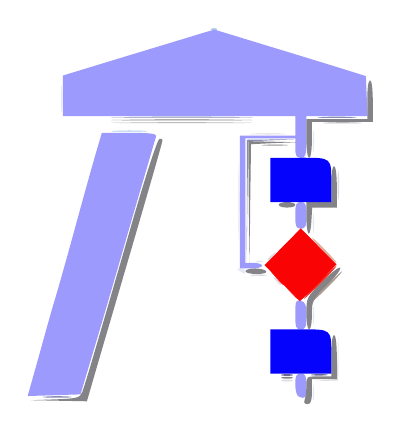
\begin{tikzpicture}[
        y = 0.1pt,
        x = 0.1pt,
        yscale = -1,
        xscale = 1,
    ]
        \begin{scope}[fill = ce5e8f5]
            \path[fill] (1043,1330) .. controls (1043,1305) and   (1045,1295) .. (1047,1308) .. controls   (1049,1320) and (1049,1340) .. (1047,1353) ..   controls (1045,1365) and (1043,1355) ..   (1043,1330) -- cycle;
            \path[fill] (1043,1050) .. controls (1043,1020) and   (1045,1007) .. (1047,1023) .. controls   (1049,1038) and (1049,1062) .. (1047,1078) ..   controls (1045,1093) and (1043,1080) ..   (1043,1050) -- cycle;
            \path[fill] (780,890) .. controls (767,882) and   (768,880) .. (783,880) .. controls (792,880) and   (800,885) .. (800,890) .. controls (800,902) and   (799,902) .. (780,890) -- cycle;
            \path[fill] (774,640) .. controls (774,516) and   (776,466) .. (777,528) .. controls (779,589) and   (779,691) .. (777,753) .. controls (776,814) and   (774,764) .. (774,640) -- cycle;
            \path[fill] (838,853) .. controls (844,851) and   (856,851) .. (863,853) .. controls (869,856) and   (864,858) .. (850,858) .. controls (836,858) and   (831,856) .. (838,853) -- cycle;
            \path[fill] (1043,715) .. controls (1043,682) and   (1045,670) .. (1047,688) .. controls (1049,706)   and (1049,733) .. (1047,748) .. controls   (1045,763) and (1043,748) .. (1043,715) --   cycle;
            \path[fill] (1043,420) .. controls (1043,384) and   (1045,370) .. (1047,388) .. controls (1049,405)   and (1049,435) .. (1047,453) .. controls   (1045,470) and (1043,456) .. (1043,420) --   cycle;
            \path[fill] (133,265) .. controls (133,221) and   (135,204) .. (137,228) .. controls (139,251) and   (139,287) .. (137,308) .. controls (135,328) and   (133,309) .. (133,265) -- cycle;
        \end{scope}
        \begin{scope}[fill = cdfdbe2]
            \path[fill] (933,1283) .. controls (942,1281) and (958,1281) .. (968,1283) .. controls (977,1286) and (969,1288) .. (950,1288) .. controls (931,1288) and (923,1286) .. (933,1283) -- cycle;
            \path[fill] (1090,1283) -- (1129,1279) -- (1133,1202) -- (1136,1125) -- (1136,1205) -- (1135,1285) -- (1092,1286) -- (1050,1287) -- (1090,1283) -- cycle;
            \path[fill] (909,923) .. controls (896,907) and (897,906) .. (913,919) .. controls (922,926) and (930,934) .. (930,936) .. controls (930,944) and (922,939) .. (909,923) -- cycle;
            \path[fill] (823,903) .. controls (838,901) and (860,901) .. (873,903) .. controls (885,905) and (873,907) .. (845,907) .. controls (818,907) and (807,905) .. (823,903) -- cycle;
            \path[fill] (880,846) .. controls (880,844) and (888,836) .. (898,829) .. controls (913,816) and (914,817) .. (901,833) .. controls (888,849) and (880,854) .. (880,846) -- cycle;
            \path[fill] (1133,580) .. controls (1133,533) and (1135,514) .. (1137,538) .. controls (1139,561) and (1139,599) .. (1137,623) .. controls (1135,646) and (1133,627) .. (1133,580) -- cycle;
            \path[fill=cdfdbe2] (828,393) .. controls (856,391) and (904,391) .. (933,393) .. controls (961,395) and (938,396) .. (880,396) .. controls (822,396) and (799,395) .. (828,393) -- cycle;
            \end{scope}
        \begin{scope}[fill = cafcde9]
            \path[fill] (328,383) .. controls (356,381) and (404,381) .. (433,383) .. controls (461,385) and (438,386) .. (380,386) .. controls (322,386) and (299,385) .. (328,383) -- cycle;
            \path[fill] (678,13) .. controls (685,10) and (694,11) .. (697,14) .. controls (701,17) and (695,20) .. (684,19) .. controls (673,19) and (670,16) .. (678,13) -- cycle;
        \end{scope}
        \begin{scope}[fill = c9c9afc]
            \path[fill] (993,1343) .. controls (985,1341) and (980,1321) .. (980,1299) .. controls (980,1267) and (983,1260) .. (1000,1260) .. controls (1017,1260) and (1020,1267) .. (1020,1305) .. controls (1020,1349) and (1017,1353) .. (993,1343) -- cycle;
            \path[fill] (56,1188) .. controls (79,1104) and (103,1019) .. (109,1000) .. controls (115,981) and (148,866) .. (181,745) .. controls (214,624) and (250,495) .. (261,458) -- (281,390) -- (381,390) .. controls (458,390) and (481,393) .. (477,403) .. controls (475,409) and (436,543) .. (390,700) .. controls (345,857) and (285,1064) .. (256,1160) -- (204,1335) -- (108,1338) -- (13,1341) -- (56,1188) -- cycle;
            \path[fill] (980,1046) .. controls (980,997) and (982,992) .. (1000,997) .. controls (1017,1001) and (1020,1011) .. (1020,1051) .. controls (1020,1093) and (1017,1100) .. (1000,1100) .. controls (982,1100) and (980,1093) .. (980,1046) -- cycle;
            \path[fill] (780,640) -- (780,400) -- (880,400) -- (980,400) -- (980,365) -- (980,330) -- (560,330) -- (140,330) -- (140,257) -- (140,183) -- (363,115) .. controls (485,78) and (608,41) .. (636,32) -- (688,17) -- (891,79) .. controls (1003,113) and (1127,151) .. (1165,163) -- (1235,185) -- (1238,258) -- (1241,330) -- (1130,330) -- (1020,330) -- (1020,405) .. controls (1020,473) and (1018,480) .. (1000,480) .. controls (984,480) and (980,473) .. (980,445) -- (980,410) -- (890,410) -- (800,410) -- (800,635) -- (800,860) -- (830,860) .. controls (847,860) and (860,865) .. (860,870) .. controls (860,876) and (842,880) .. (820,880) -- (780,880) -- (780,640) -- cycle;
            \path[fill] (980,688) .. controls (980,647) and (983,640) .. (1000,640) .. controls (1017,640) and (1020,647) .. (1020,688) .. controls (1020,729) and (1017,736) .. (1000,736) .. controls (983,736) and (980,729) .. (980,688) -- cycle;
        \end{scope}
        \begin{scope}[fill = cb9babc]
            \path[fill] (868,433) .. controls (891,431) and (927,431) .. (948,433) .. controls (968,435) and (949,437) .. (905,437) .. controls (861,437) and (844,435) .. (868,433) -- cycle;
            \path[fill] (363,353) .. controls (477,351) and (663,351) .. (778,353) .. controls (892,354) and (798,355) .. (570,355) .. controls (342,355) and (248,354) .. (363,353) -- cycle;
            \path[fill] (1093,353) .. controls (1124,351) and (1176,351) .. (1208,353) .. controls (1239,355) and (1213,356) .. (1150,356) .. controls (1087,356) and (1061,355) .. (1093,353) -- cycle;
        \end{scope}
        \begin{scope}[fill = cddae9b]
            \path[fill] (1080,815) .. controls (1056,790) and (1038,770) .. (1041,770) .. controls (1044,770) and (1066,790) .. (1090,815) .. controls (1114,840) and (1132,860) .. (1129,860) .. controls (1126,860) and (1104,840) .. (1080,815) -- cycle;
        \end{scope}
        \begin{scope}[fill = cf8776f]
            \path[fill] (959,963) -- (935,935) -- (963,959) .. controls (988,982) and (995,990) .. (987,990) .. controls (985,990) and (973,978) .. (959,963) -- cycle;
        \end{scope}
        \begin{scope}[fill = cac9b8b]
            \path[fill] (1090,945) .. controls (1120,915) and (1147,890) .. (1149,890) .. controls (1152,890) and (1130,915) .. (1100,945) .. controls (1070,975) and (1043,1000) .. (1041,1000) .. controls (1038,1000) and (1060,975) .. (1090,945) -- cycle;
        \end{scope}
        \begin{scope}[fill = c878cb9]
            \path[fill] (77,1343) .. controls (101,1341) and (139,1341) .. (162,1343) .. controls (186,1345) and (167,1347) .. (120,1347) .. controls (73,1347) and (54,1345) .. (77,1343) -- cycle;
            \path[fill] (805,635) -- (805,415) -- (890,414) -- (975,414) -- (893,417) -- (810,421) -- (807,638) -- (804,855) -- (805,635) -- cycle;
            \path[fill] (363,333) .. controls (477,331) and (663,331) .. (778,333) .. controls (892,334) and (798,335) .. (570,335) .. controls (342,335) and (248,334) .. (363,333) -- cycle;
            \path[fill] (1073,333) .. controls (1104,331) and (1156,331) .. (1188,333) .. controls (1219,335) and (1193,336) .. (1130,336) .. controls (1067,336) and (1041,335) .. (1073,333) -- cycle;
        \end{scope}
        \begin{scope}[fill = c848387]
            \path[fill] (1014,1354) .. controls (1017,1345) and (1020,1323) .. (1020,1304) .. controls (1020,1270) and (1020,1270) .. (1065,1270) -- (1110,1270) -- (1110,1195) .. controls (1110,1152) and (1114,1120) .. (1120,1120) .. controls (1126,1120) and (1130,1153) .. (1130,1200) -- (1130,1280) -- (1085,1280) -- (1040,1280) -- (1040,1325) .. controls (1040,1360) and (1036,1370) .. (1024,1370) .. controls (1013,1370) and (1010,1365) .. (1014,1354) -- cycle;
            \path[fill] (113,1353) .. controls (193,1350) and (202,1347) .. (210,1327) .. controls (219,1304) and (247,1211) .. (393,705) .. controls (439,546) and (482,414) .. (489,412) .. controls (495,410) and (500,412) .. (500,417) .. controls (500,425) and (422,694) .. (274,1198) -- (227,1360) -- (126,1358) -- (25,1356) -- (113,1353) -- cycle;
            \path[fill] (933,1273) .. controls (942,1271) and (958,1271) .. (968,1273) .. controls (977,1276) and (969,1278) .. (950,1278) .. controls (931,1278) and (923,1276) .. (933,1273) -- cycle;
            \path[fill] (1020,1042) .. controls (1020,985) and (1021,984) .. (1079,926) .. controls (1111,894) and (1140,872) .. (1143,877) .. controls (1146,882) and (1125,911) .. (1095,940) .. controls (1042,992) and (1040,996) .. (1040,1047) .. controls (1040,1076) and (1036,1100) .. (1030,1100) .. controls (1024,1100) and (1020,1074) .. (1020,1042) -- cycle;
            \path[fill] (800,890) .. controls (800,885) and (815,880) .. (834,880) .. controls (853,880) and (872,885) .. (875,890) .. controls (879,896) and (865,900) .. (841,900) .. controls (818,900) and (800,896) .. (800,890) -- cycle;
            \path[fill] (812,643) -- (810,420) -- (898,422) -- (985,424) -- (903,427) -- (820,431) -- (817,648) -- (815,865) -- (812,643) -- cycle;
            \path[fill] (1028,754) .. controls (1023,750) and (1020,723) .. (1020,693) -- (1020,640) -- (1065,640) -- (1110,640) -- (1110,575) .. controls (1110,538) and (1114,510) .. (1120,510) .. controls (1126,510) and (1130,542) .. (1130,585) -- (1130,660) -- (1086,660) -- (1041,660) -- (1038,711) .. controls (1036,739) and (1032,758) .. (1028,754) -- cycle;
            \path[fill] (920,650) .. controls (920,645) and (934,640) .. (950,640) .. controls (967,640) and (980,645) .. (980,650) .. controls (980,656) and (967,660) .. (950,660) .. controls (934,660) and (920,656) .. (920,650) -- cycle;
            \path[fill] (1020,410) -- (1020,340) -- (1130,340) -- (1240,340) -- (1240,270) .. controls (1240,230) and (1244,200) .. (1250,200) .. controls (1256,200) and (1260,232) .. (1260,275) -- (1260,350) -- (1150,350) -- (1040,350) -- (1040,415) .. controls (1040,452) and (1036,480) .. (1030,480) .. controls (1024,480) and (1020,450) .. (1020,410) -- cycle;
            \path[fill] (363,343) .. controls (477,341) and (663,341) .. (778,343) .. controls (892,344) and (798,345) .. (570,345) .. controls (342,345) and (248,344) .. (363,343) -- cycle;
        \end{scope}
        \begin{scope}[fill = c6c6898]
            \path[fill] (933,1263) .. controls (942,1261) and (958,1261) .. (968,1263) .. controls (977,1266) and (969,1268) .. (950,1268) .. controls (931,1268) and (923,1266) .. (933,1263) -- cycle;
            \path[fill] (1043,1263) .. controls (1058,1261) and (1080,1261) .. (1093,1263) .. controls (1105,1265) and (1093,1267) .. (1065,1267) .. controls (1038,1267) and (1027,1265) .. (1043,1263) -- cycle;
        \end{scope}
        \begin{scope}[fill = cf52d21]
            \path[fill] (1065,930) .. controls (1098,897) and (1127,870) .. (1129,870) .. controls (1132,870) and (1108,897) .. (1075,930) .. controls (1042,963) and (1013,990) .. (1011,990) .. controls (1008,990) and (1032,963) .. (1065,930) -- cycle;
            \path[fill] (914,918) -- (895,895) -- (918,914) .. controls (939,932) and (945,940) .. (937,940) .. controls (935,940) and (925,930) .. (914,918) -- cycle;
        \end{scope}
        \begin{scope}[fill = c0503fc]
            \path[fill] (890,1180) -- (890,1100) -- (994,1100) .. controls (1114,1100) and (1110,1097) .. (1110,1196) -- (1110,1260) -- (1000,1260) -- (890,1260) -- (890,1180) -- cycle;
            \path[fill] (890,560) -- (890,480) -- (994,480) .. controls (1114,480) and (1110,477) .. (1110,576) -- (1110,640) -- (1000,640) -- (890,640) -- (890,560) -- cycle;
        \end{scope}
        \begin{scope}[fill = cfa0305]
            \path[fill] (932,933) -- (869,868) -- (934,802) -- (1000,735) -- (1064,800) -- (1129,865) -- (1064,933) .. controls (1027,970) and (997,999) .. (996,998) .. controls (996,998) and (967,968) .. (932,933) -- cycle;
        \end{scope}

    \end{tikzpicture}
}

% Colors needed for the logo (sketchy) of the Department of Computer Science of the University of Kaiserslautern
\definecolor{c808080}{RGB}{128,128,128}
\definecolor{cff0000}{RGB}{255,0,0}
\definecolor{c9999ff}{RGB}{153,153,255}
\definecolor{c0000ff}{RGB}{0,0,255}

% The logo of the Department of Computer Science of the University of Kaiserslautern:
% Taken from: http://sci.informatik.uni-kl.de/rechnerzugang/terminals/lageplan_sci/Lageplan_SCI.pdf on the 2017-03-16
% Manipulated using: Inkscape (https://inkscape.org/)
% Converted to TikZ using: svg2tikz (https://github.com/kjellmf/svg2tikz) as an Inkscape extension
\newcommand{\CSLogo}{
    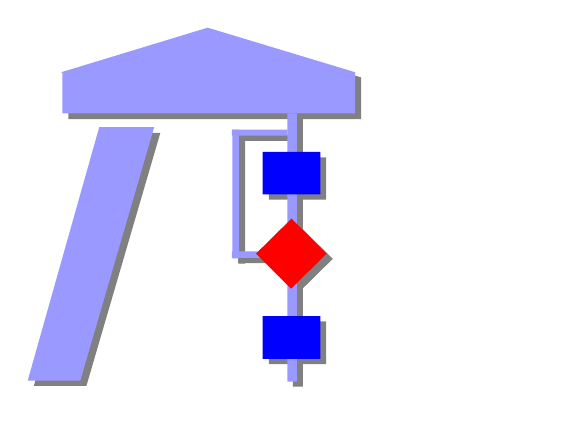
\begin{tikzpicture}[
        y = 1.65pt,
        x = 1.65pt,
        yscale = -1,
        xscale = 1
    ]
        \begin{scope}[cm={{0.0, 1.25, 1.25, 0.0, (-153.75, -108.75)}}]
            \path[cm = {{0.0, 0.82808, 1.0, 0.0, (125.0216, 604.3906)}}, fill = c808080, nonzero rule] (0.0000, 0.0000) node[above right] (text2307) {};
            \path[cm = {{0.0, 0.82379, 1.0, 0.0, (125.0216, 609.1211)}}, fill = c808080, nonzero rule] (0.0000, 0.0000) node[above right] (text2311) {};
            \path[cm = {{0.0, 0.82808, 1.0, 0.0, (145.8526, 604.3906)}}, fill = c808080, nonzero rule] (0.0000, 0.0000) node[above right] (text2315) {};
            \path[cm = {{0.0, 0.82379, 1.0, 0.0, (145.8526, 609.1211)}}, fill = c808080, nonzero rule] (0.0000, 0.0000) node[above right] (text2319) {};
            \path[cm = {{0.0, 0.75, 1.0, 0.0, (168.3434, 604.3906)}}, fill = c808080, nonzero rule] (0.0000, 0.0000) node[above right] (text2323) {};
            \path[cm = {{0.0, 1.0, 0.97692, 0.0, (125.1046, 587.6261)}}, fill = c808080, nonzero rule] (0.0000, 0.0000) node[above right] (text2327) {};
            \path[cm = {{0.0, 1.0, 0.95143, 0.0, (147.0145, 587.3771)}}, fill = c808080, nonzero rule] (0.0000, 0.0000) node[above right] (text2331) {};
            \path[cm = {{0.0, 1.0, 0.62474, 0.0, (169.6713, 591.1118)}}, fill = c808080, nonzero rule] (0.0000, 0.0000) node[above right] (text2355) {};
            \path[cm = {{0.0, 1.0, 0.97692, 0.0, (123.8597, 585.9662)}}, fill = cff0000, nonzero rule] (0.0000, 0.0000) node[above right] (text2379) {};
            \path[cm = {{0.0, 1.0, 0.95143, 0.0, (145.8526, 585.7173)}}, fill = cff0000, nonzero rule] (0.0000, 0.0000) node[above right] (text2383) {};
            \path[cm = {{0.0, 1.0, 0.62474, 0.0, (168.5094, 589.452)}}, fill = cff0000, nonzero rule] (0.0000, 0.0000) node[above right] (text2407) {};
            \path[fill = c808080, even odd rule] (123.5280, 563.8070) -- (123.5280, 558.9940) -- (122.4490, 558.9940) -- (122.4490, 568.6210) -- (123.5280, 568.6210) -- (123.5280, 563.8070);
            \path[fill = c808080, even odd rule] (144.9400, 563.8070) -- (144.9400, 558.9940) -- (143.7780, 558.9940) -- (143.7780, 568.6210) -- (144.9400, 568.6210) -- (144.9400, 563.8070);
            \path[fill = c808080, even odd rule] (133.7360, 559.0770) -- (122.4490, 559.0770) -- (122.4490, 560.2390) -- (145.0230, 560.2390) -- (145.0230, 559.0770) -- (133.7360, 559.0770);
            \path[fill = c808080, even odd rule] (143.1970, 568.6210) -- (119.7100, 568.6210) -- (119.7100, 570.3640) -- (166.6010, 570.3640) -- (166.6010, 568.6210) -- (143.1970, 568.6210);
            \path[fill = c808080, even odd rule] (112.4070, 529.1170) -- (104.6890, 554.7610) -- (112.4070, 580.5720) -- (119.7100, 580.5720) -- (119.7100, 529.2830) -- (112.4070, 529.2830) -- (112.5730, 529.1170) -- (112.4070, 529.1170);
            \path[fill = c808080, even odd rule] (122.1170, 535.7560) -- (122.1170, 545.3830) -- (166.4350, 532.4360) -- (166.4350, 523.2240) -- (122.1170, 535.7560);
            \path[fill = c808080, even odd rule] (147.2630, 566.2970) -- (144.2760, 563.2260) -- (138.1340, 569.4510) -- (144.1930, 575.5920) -- (150.3340, 569.3680) -- (147.2630, 566.2970);
            \path[fill = c808080, even odd rule] (133.8190, 569.4510) -- (133.8190, 564.3880) -- (126.4320, 564.3880) -- (126.4320, 574.4300) -- (133.8190, 574.4300) -- (133.8190, 569.4510);
            \path[fill = c808080, even odd rule] (162.6170, 569.4510) -- (162.6170, 564.3880) -- (155.1480, 564.3880) -- (155.1480, 574.4300) -- (162.6170, 574.4300) -- (162.6170, 569.4510);
            \path[fill = c9999ff, even odd rule] (122.6150, 562.8110) -- (122.6150, 557.9150) -- (121.5360, 557.9150) -- (121.5360, 567.6250) -- (122.6150, 567.6250) -- (122.6150, 562.8110);
            \path[fill = c9999ff, even odd rule] (144.0270, 562.8110) -- (144.0270, 557.9150) -- (142.8650, 557.9150) -- (142.8650, 567.6250) -- (144.0270, 567.6250) -- (144.0270, 562.8110);
            \path[fill = c9999ff, even odd rule] (132.8230, 557.9980) -- (121.5360, 557.9980) -- (121.5360, 559.1600) -- (144.1100, 559.1600) -- (144.1100, 557.9980) -- (132.8230, 557.9980);
            \path[fill = c9999ff, even odd rule] (142.2010, 567.6250) -- (118.7140, 567.6250) -- (118.7140, 569.2850) -- (165.6880, 569.2850) -- (165.6880, 567.6250) -- (142.2010, 567.6250);
            \path[fill = c9999ff, even odd rule] (111.4940, 528.0380) -- (103.6930, 553.6820) -- (111.4940, 579.4930) -- (118.7140, 579.4930) -- (118.7140, 528.2040) -- (111.4940, 528.2040) -- (111.6600, 528.0380) -- (111.4940, 528.0380);
            \path[fill = c9999ff, even odd rule] (121.1210, 534.6770) -- (121.1210, 544.3040) -- (165.5220, 531.3570) -- (165.5220, 522.1450) -- (121.1210, 534.6770);
            \path[fill = cff0000, even odd rule] (146.3510, 565.2180) -- (143.2800, 562.1480) -- (137.1380, 568.3720) -- (143.2800, 574.5130) -- (149.4210, 568.2890) -- (146.3510, 565.2180);
            \path[fill = c0000ff, even odd rule] (132.9060, 568.3720) -- (132.9060, 563.3090) -- (125.4370, 563.3090) -- (125.4370, 573.4340) -- (132.9060, 573.4340) -- (132.9060, 568.3720);
            \path[fill = c0000ff, even odd rule] (161.7040, 568.3720) -- (161.7040, 563.3090) -- (154.2350, 563.3090) -- (154.2350, 573.4340) -- (161.7040, 573.4340) -- (161.7040, 568.3720);
            \path[cm = {{0.0, 0.82808, 1.0, 0.0, (124.0257, 603.3947)}}, fill = c9999ff, nonzero rule] (0.0000, 0.0000) node[above right] (text2467) {};
            \path[cm = {{0.0, 0.82379, 1.0, 0.0, (124.0257, 608.1252)}}, fill = c9999ff, nonzero rule] (0.0000, 0.0000) node[above right] (text2471) {};
            \path[cm = {{0.0, 0.82808, 1.0, 0.0, (144.8567, 603.3947)}}, fill = c9999ff, nonzero rule] (0.0000, 0.0000) node[above right] (text2475) {};
            \path[cm = {{0.0, 0.82379, 1.0, 0.0, (144.8567, 608.1252)}}, fill = c9999ff, nonzero rule] (0.0000, 0.0000) node[above right] (text2479) {};
            \path[cm = {{0.0, 0.75, 1.0, 0.0, (167.4305, 603.3947)}}, fill = c0000ff, nonzero rule] (0.0000, 0.0000) node[above right] (text2483) {};
        \end{scope}

    \end{tikzpicture}
}
